\chapter{Design}
\label{chap:design}

\section{Introduction}
\label{sec:designintroduction}

The goal of this thesis is to develop a modularized and production grade user simulator that can be re-targeted for new domains and provide a framework to produce training data and train dialog agents. The overall design for the simulator was inspired by the work done by \cite{li_usersim} and the formalization of hidden user agenda models by \cite{Schatzmann2009TheHA}. 

Underlying the simulator is a framework that consists the following components:
\begin{itemize}
	\item \textbf{User Simulator}: An agenda based user modeling component that generates natural language speech utterances to simulate what an actual human would say in the context of task-completion dialog activity. 
	\item \textbf{Dialog Agent API}: A set of methods to allow a researcher to provide an agent(s) that simulate how the system / dialog agent would respond 
	\item \textbf{Dialog Manager}: A coordinator component that tracks the current state of the dialog and facilitates the conversation between the user simulator and dialog agent/system. Add the end of the simulated conversation, the manager will evaluate and score the conversion. 
\end{itemize}

\section{User Simulator} 

The user simulator is responsible for imitating a real user and generating realistic speech utterances. Here we assume the user is an actor that is attempting complete task. For example, the user may want to travel to Japan and is attempting to book a flight there. That user could then interact with a travel agent chatbot in order to get assistance in identifying the appropriate flight and purchasing tickets. In order to model and represent a user, we will utilize the formalization of the hidden user agenda described in \cite{Schatzmann2009TheHA}.

 One of the primary assumptions here is that user has intentionally engaged with the dialog agent in order to complete their task. At the outset of the conversation, the user will have some specific goal in mind (order Indian food, book a flight to Japan, etc). The dialog agent will attempt to learn user's goal by asking the user a set of clarifying questions. Schatzmann and Young introduces the idea of a hidden user agenda as a mechanism to represent the sequence of dialog acts and utterances a user will say in the context of that conversation. At each step of a task-completion dialog, the user is either responding to the dialog agent or initiating a new conversation direction. The user agenda provides an efficient way and formal structure to represent the pending set of dialog acts the user will communicate to the dialog agent.
 
Socrates Simulator implements the Schatzmann and Young's concept of user agenda and user goal as first class objects. The conversion from the formal representation to code is rather straightforward as there are analogous data structures. We will defer discussing implementation details until the next chapter. The subsections below will further describe how the user goal and agenda is defined. 

\subsection{User Goals} 
The user goal captures explicitly both user's preferences and missing information needs they are trying to fill. For example, take a user who wants to find an Indian restaurant in Central square for dinner. We can decompose this goal into two distinct components. The first is the user's explicit preferences. In this example, their preferred cuisine is Indian. The second component is implicit and unknown to the user. They are looking for a restaurant or more specifically the name and presumably the restaurant's phone number and address. This information is unknown but can be broken down into discrete pieces of information the user will attempt to elicit from the dialog agent as a request for more information. 

Formally, Schatzmann and Young defines the user goal \textit{G} as \textit{G = (C,R)}, where \textit{C} consists of constraints or the user's explicit preferences and \textit{R} represents the user's requests. The constraints and requests are explicitly represented as slot-value pairs. \ref{fig:goals1} below shows how one could represent the goal of user looking for a bar. 

\begin{figure}[h!]
	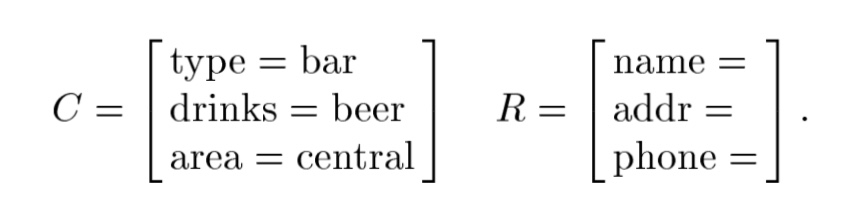
\includegraphics[width=\linewidth]{diagrams/schatzmann_goal_fig.jpeg}
	\caption{Example User goal. User wants the name, address and phone number of a cheap bar in central.  }
	\label{fig:goals1}
\end{figure}

The concept of a goal abstractly turns out to be useful in also driving the dialog manager's simulations. We abstract the idea of goal and make it available to both the user and dialog agent api as way to track the internal state of each speaker. 

\subsection{User Agenda} 

Schatzmann and Young define the user agenda as a “[stack] structure of pending dialogue acts [which] serve as a convenient mechanisms for encoding the dialogue history and user’s ‘state of mind’ ” \cite{Schatzmann2009TheHA}. Formally, at any time t, the user is in a state su  and takes an action au,which transitions into an intermediate state s’u. During this intermediate state, the user will receive an action from the system (machine) am, which will transition dialog to next state s’’u and the cycle will reset. The result is a sequence of alternating turns between the user and system (i.e. su -> au -> s’u -> am -> s’’u -> … ), which represents the conversation state over time t.
 
The user agenda A is stack-like structure which contains all pending user actions. User actions are actualized through popping the stack and the agenda is updated by pushing back onto the stack. A user act is a representation of the user’s intent, which will eventually be translated into a speech utterance. The stack may also contain other actions that will affect the user when popped. For example, the system can communicate a restaurant suggestion, which would fill the one of the request slots for restaurant name.  

At the start of the dialog a new goal is randomly generated from the provided dialog domain. An accompanying agenda is then generated to represent the potential sequential of events. 

Below is an  example of the a sample user agenda that Schatzmann and Young provide in the context of a user asking the dialog system for a bar recommendation [6]. The states of the conversation are indexed by time t. Note, Schatzmann and Young use constraints C, which would be the equivalent of inform slots in our representation. In the first turn, the user simulator generates a set of constraints (bar serving beer in central) and goals (name, address, and phone for a bar that meets the constraints in C0). This set of inform and request slots are translated into a user action stored in A0. When the system initiates the conversation, the user simulator pops two inform actions which translate into the user utterance “I’m looking for a nice bar serving beer”. When the system at t=1, responds “Ok, a wine bar. What price range?” the agenda updated to include a new inform intent (inform(prange=cheap)). Also added is a negate action, as the user asked beer and not wine. 

Over the course of the conversation the agenda is updated, as are the request slots. The conversation ends at t=5, when bye() is popped and the agenda stack is empty. The conversation will then be evaluated based on how well the request slots were filled.



\section{Dialog Model}

\subsection{Overview}

Add paragraph here about high level design and how all component fit together. 

Give example of simple conversation flow.


\subsection{Design Philosophy}

At a high level, our aim is to develop a framework to allow dialog researchers to simulate a conversation between the user simulator and dialog agent. The framework needs to be modular so that it can be quickly adapted to support new dialog domains and experiments. Each major component of the framework is represented as a python class. Additionally, I promoted dialog actions, goals, and domain knowledge bases to first class objects, rather than implementing them at the lower dictionary level. As first class objects, I can standardize the communication, APIs, and management of these pieces and ensure more consistent behavior.

Additionally, we want to provide as much flexibility and freedom to the researcher and limit what is hard-coded. I follow the configuration first approach leveraged in the development of AllenNLP, a deep learning for NLP tool developed at the Allen Institute for Artificial Intelligence. The code is generalized and the user defines particular implementation details in configuration file. To support a configuration driven approach, each configurable module will have a use defined yaml or json file. For smaller configuration details, the user will prefer using yaml which is more human readable. The yaml format is simple and has a very low learning curve. It follows a basic key value pair paradigm, where keys have clear semantic meaning and values can be represented in a variety of data structures. 

\begin{figure}[h!]
	\caption{Example yaml section. }
	\label{fig:ex_yaml}
	\begin{lstlisting}
		# Dialog Simulation settings
		simulation_rounds: 10
		max_turns: 8
		first_speaker: usersim
		reward: 10
		simulation_output_path: data/simulated_dialogs/
		save_history: True
		save_location: "data/simulated_dialogs/"
		save_type: json
	\end{lstlisting}
\end{figure}

\section{ Framework Overview}

All components are represented as python classes. The ensuing section further describe the component's function, design, and any salient implementation details. 

\subsection{Dialog  Manager}

The Dialog Manager class does thing

\subsection{Dialog Action}

The fundamental unit of transaction for the simulator is the dialog action. It is an explicit semantic representation of the speech utterance that is machine readable. For example, I could represent the speech utterance, "I'm looking for a  Thai restaurant", in the following way:
	original utterance: \textit{I'm looking for a Thai restaurant}
	dialog act: \textit{request}
	constraints: \textit{cuisine=Thai}
The DialogAction object standardizes and encodes information about a speech act that can be understood by both the user simulator and dialog agent. The dialog action consist of three key properties: the dialog act, a set of explicit dialog parameters or constraints, and corresponding unparsed speech utterance. I will next describe these properties in further detail. 

The unparsed speech utterance is just the natural language utterance that was spoken by the feature. One of the goals of the user simulator is to generate speech utterances based off its internal user agenda. The user simulator will use the dialog act and dialog parameters popped from the user agenda to generate a new utterance using it natural language generation model. If a speaker is hearing the utterance, then the utterance will need to be parsed and broken into a dialog action and set of dialog parameters in ordered to be processed. 

The dialog act property is used to capture the intent of the speech act. Common dialog acts include: inform, request, confirm, negate, and affirm. The dialog act is necessary to provide context for the dialog parameters for both the natural language generation and understanding use cases. For example, a set of dialog parameters like "{cuisine=thai, area=north}" can be interpreted differently in the inform vs request context. In the request context, the speech utterance could be "I'd like to find a thai restaurant in north part of town". In contrast, those same dialog parameters could be part of a suggestion in the inform context. E.g. "There is a great Thai restaurant in the north part of town". Given the variability of dialog acts and intents, the space of possible dialog acts is defined by the researcher in a configuration file. While this limits the possible interpretations of the speech act, a reduced dialog act space is vital to building effective task completion dialog agents.  

As we saw above, the dialog parameters encode entities in the speech utterance as key-value pairs and are used the communicate  or elicit the user's preferences. The key captures the entity type or constraint type (e.g. cuisine, area, address, etc), while the value is used to indicate the specific constraint or entity (e.g. Thai, north, 115 Way Street, etc). The parameter property is strictly typed as a python dictionary and therefore all keys must be associated with a value. In the context of request speech acts, the null value is used to indicate the speaker wants to elicit more information the provided constraint type. For example, \textit{dialog\_act=request, params=\{address: NULL\}}, would be interpreted as a request for the address (e.g."What is the address?"). 

Initially, I used python dictionaries and sets to represent the dialog parameters. However, this was as an sub-optimal several reasons. First it introduced variability and uncertainty. To capture request parameters I used python sets, since the value was null and we justed needed to pass along the constraints types. For all dialog actions, I used explicit dictionaries as real values were passed along with the constrain types. However, downstream this required logic to check the class instance of the parameter variable being passed in. Given the dynamical nature of the dialogs being generated, the simulator was rather unstable and would randomly crash due when a method expecting a dictionary, received a set. By enforcing a the python dictionary type and setting null values, I was able to greatly improve stability and make debugging easier by standardizing the input into functions that consumed the DialogAction object. 

\subsection{Goals}

The Goal class represents the objective of the speaker at the outset of the conversation. For the user simulator, the goal defines the hidden set of preferences and information needs the user has. The goal object has two properties, the inform slots and request slots. Both the inform and request slots are typed as python dictionaries.The inform slots capture the user's preferences that they want to communicate to the dialog agent. A well developed dialog agent should be able to elicit those preferences efficiently and ideally without needing to ask the user multiple times. The request slots capture the information user needs in order to complete their objective and task. At the start of the conversation, all the request slots values are set to null values. Over the course of the dialog, as the dialog agent responds the user simulator, the request slots may be updated with real values. A dialog is considered successful if all the request slots for the user simulator have been replaced by real values. The user simulator monitors the state of the request slots in it Goal object. If all the request slots are filled, the user simulator update its internal dialog status to the complete state and signal to the dialog manager to end the conversation. 

In the first iteration, only the user simulator had a Goal object. But it made sense to include the Goal object for the dialog agent as well. The rationale behind this was two-fold. First it provided a useful mechanism to track the state of the dialog agent as well. Like the user, the dialog agent has its own set of goal, i.e. to elicit the information it needs to provide a meaningful suggestion or provide the specific service the user desires. The request slots in the dialog agent are complimentary to the user's inform slots. Ideally, the dialog agent will effectively elicit the user inform slot through a series of request speech acts and then execute it service. This leads us to the second value for the dialog agent, the Goal object provided a useful mechanism for training (especially in the reinforcement learning context). In failure cases, it signals to the researcher the information the dialog agent was ineffective at capturing. For reinforcement learning, a loss function can be developed that minimize the open request slots in the agent's Goal at the end of each conversation when the agent renders its service. 

\subsection{Dialog Status}

The DialogStatus is a python enumerative object that encodes the internal state of the dialog for each speaker. Each speaker is responsible for setting its own dialog status. The valid states are not started, no outcome yet and finished. The dialog manager will probe each speaker for it's dialog state. It the dialog manager learns that the state for any speaker is set to finished, the conversation will be ended. The user simulator sets its dialog status to finished when all the requests slots in it Goal object are filled. In contrast the dialog agent may only set its state to finished after the user leaves the conversation. This way the agent does not prematurely exit the conversation before the user can complete their task. 

\subsection{Speaker}

The speaker represents an actor that has the ability to speak and comprehend speech utterances. In our framework, the both user simulator and the dialog agent are represented by the same base speaker class. Both actors conceptually are identical in terms of functional behavior, in that they both listen and comprehend speech utterances and in turn respond by speaking. As such, both the user simulator and dialog agent can be represented in the same way to the dialog manager. In fact, the entire conversation round can be expressed in two lines: 

\begin{figure}[h!]
	\caption{Psuedo code for conversation round.}
	\label{fig:conv_round}
	\begin{lstlisting}
	# Assuming user speaks first 
	# 1. User Simulator takes turn and speaks
	user_action = user_simulator.next(previous_agent_action, turn_number)
	# 2. Agent takes turn and responds to user 
	agent_action = agent.next(previous_user_action, turn_number)
	\end{lstlisting}
\end{figure}

The speaker class has four basic functions (\textit{next, reset, get utterance, and parse utterance}) and three properties (\textit{nlg model, nlu model, and dialog status}). When the speaker is initialized, the natural language object and the natural language understanding object are passed to the constructor. We abstract away the implementation of how the speaker speaks and parses speech in order maintain separation of concerns and also empower the researcher to be able to experiment with multiple techniques. 

The \textit{next} method is the primary driver how the speaker behaves. For the dialog agent class, the next method functions as an API to the simulator. It is assumed that the dialog agent will live and operate external the simulator. The researcher can define how the dialog agent will interact with the user simulator here. For the user simulator, the bulk of the logic will reside here. The \textit{get utterance} and \textit{parse utterances} methods are simply wrappers for the speaker's nlg and nlg objects. The primary parameter for next is the previous dialog action. 

\begin{figure}[h!]
	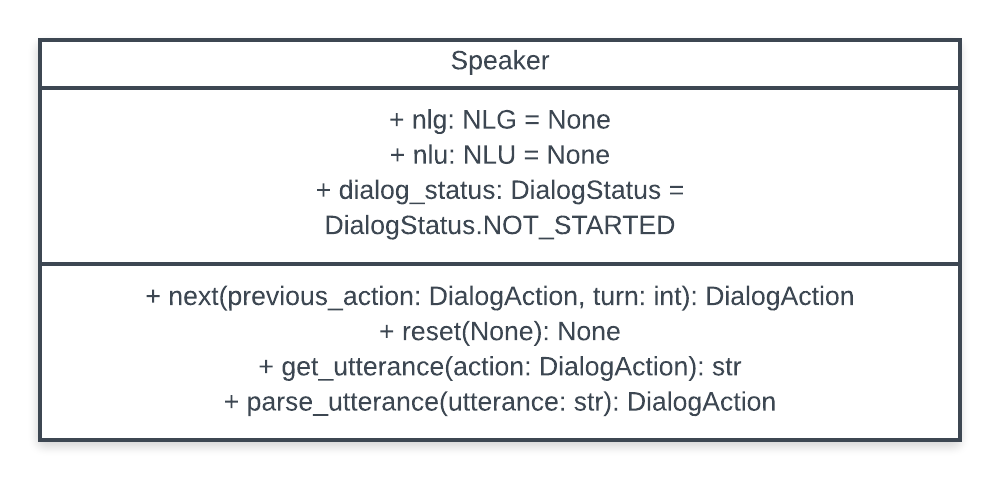
\includegraphics[width=\linewidth]{diagrams/speaker_class.png}
	\caption{ Definition of the Speaker class and methods.}
	\label{fig:speaker_class}
\end{figure}


\subsection{Dialog Domain and Domain Knowledge Base}

The domain class standardizes the collection and storage of information related to domain of the services provided by the dialog agent. The domain class is initialized by a configuration file defined by the researcher and provides a set of APIs to access dialog domain elements. The domain class consists of the following key properties: dialog acts, request slots, inform slots and inform slot values, valid user goals templates, sample starting goals list, and a domain knowledge base object.  Additionally the following key API methods are made available: sample inform slots and inform slot values, sample request slots, get valid user goals, and get suggestions (from domain knowledge base) and validate suggestions. 

The primary consumer of the domain class is the dialog manager, which uses the domain information to generate new user goals or sample user goals from a preexisting list of starting goals. If the dialog manager is generating novel user goals, it will use the valid user goals template to create a new goal and sample the inform slots to generate the user's preferences for that goal. 

The domain knowledge base (KB) is modeled as a distinct class and serves as an interface to a knowledge base / database the dialog agent would have access to. The primary purpose of the domain KB is store all the suggestions that a dialog agent would make based on the various preferences of the user. The domain KB provides an interface with the following three methods; get suggestions, validate suggestions, and get item. The researcher is free to use whichever back-end and implementation to resolve those three API calls. For this thesis, I chose to use a Pandas dataframe which is an efficient in memory data table that can queried and manipulated. In the implementation section, I'll further describe my approach for resolving user queries and providing simple suggestions with greedy preference matching. 

\subsection{Natural Language Understanding (NLU) and Natural Language Generation (NLG)}

The NLU interface provides a common API for the parsing of speech utterances for each speaker. It is an interface with one API method: parse utterance. Parse utterance will take in a natural language speech utterance and return a DialogAction object. The researcher has flexibility in setting up the NLU back-end. The NLG module is a complimentary interface, and also contains a single API method: get utterance. Get utterance takes in a DialogAction object and will generate a new speech utterance.  In implementation section, we will further details the simple rules based approach and neural machine translation implementations for both the nlg and nlu back-ends. 

Upon initialization, the speaker class will set an internal nlg and nlu object. The speaker's\textit{ get\_utterance } and \textit{parse\_utterance} will directly call the correspond methods in the nlg and nlu object. This way the dialog manager does not need to know the internals of each speaker's nlg and nlu objects. 

NLU and NLOG is an open problem space and there are no single universal solutions. In abstracting the NLU and NLG interfaces, the researcher has more flexibility in training and experimenting with their dialog agent. Since the user simulator will always return the machine readable DialogAction with the generated speech utterance, the researcher has the ability to train the NLU for their dialog agent to support more robust NLU use cases. 






%%% Local Variables: 
%%% mode: latex
%%% TeX-master: "main"
%%% End: 
